%%%%%%%%%%%%%%%%%%%%%%%%%%%%%%%%%%%%%%%%%%%%%%%%%%%%%%%%%%%%%%%%
%%%%%%%%%%%%%%%%%%%%%%%%%%%%%%%%%%%%%%%%%%%%%%%%%%%%%%%%%%%%%%%%
%%%%
%%%% This text file is part of the source of slides for
%%%% `Introduction to High-Performance Scientific Computing'
%%%% by Victor Eijkhout, copyright 2012
%%%%
%%%%%%%%%%%%%%%%%%%%%%%%%%%%%%%%%%%%%%%%%%%%%%%%%%%%%%%%%%%%%%%%
%%%%%%%%%%%%%%%%%%%%%%%%%%%%%%%%%%%%%%%%%%%%%%%%%%%%%%%%%%%%%%%%

\documentclass[headnav]{beamer}

\newenvironment{beamdisplayeq}%
 {\begin{equation}\small}{\end{equation}}

\usepackage{beamerthemeTACC}
\parskip=.5\baselineskip plus .5\baselineskip
\event{Intro sci/tech computing}

\usepackage{amsmath,arydshln,graphicx,comment,multicol,undertilde}
\usepackage{hyperref}

\newcommand\inv{^{-1}}
\newcommand\argmin{\mathop{\mathrm{argmin}}}
\newcommand\setspan[1]{[\![#1]\!]}

\begin{document}
\title{Numerical Linear Algebra: iterative methods}
\author{Victor Eijkhout}
\date{}
\frame{\titlepage}


\frame{\frametitle{Two different approaches}
  Solve $Ax=b$

  Direct methods:
  \begin{itemize}
  \item Deterministic
  \item Exact up to machine precision
  \item Expensive (in time and space)
  \end{itemize}
  Iterative methods:
  \begin{itemize}
  \item Only approximate
  \item Cheaper in space and (possibly) time
  \item Convergence not guaranteed
  \end{itemize}
}

\frame{\frametitle{Iterative methods}
  Choose any $x_0$ and repeat
  \[ x^{k+1}=Bx^k+c \]
  until $\|x^{k+1}-x^k\|_2<\epsilon$
  or until $\frac{\|x^{k+1}-x^k\|_2}{\|x^k\|}<\epsilon$
}

\frame{\frametitle{Example of iterative solution}

 Example system
\[ \left(\begin{matrix}10&0&1\\ 1/2&7&1\\ 1&0&6\end{matrix}\right)
  \left(
    \begin{matrix}
      x_1\\ x_2\\ x_3
    \end{matrix}\right) = 
    \left(\begin{matrix}
      21\\ 9\\ 8
    \end{matrix}\right)
\]
with solution $(2,1,1)$.

 Suppose you know (physics) that solution components are roughly
  the same size, and observe the dominant size of the diagonal, then
\[ \left(\begin{matrix}10&\\ &7\\ &&6\end{matrix}\right)
  \left(
    \begin{matrix}
      x_1\\ x_2\\ x_3
    \end{matrix}\right) = 
    \left(\begin{matrix}
      21\\ 9\\ 8
    \end{matrix}\right)
\]
might be a good approximation: solution $(2.1,9/7,8/6)$.
}

\frame{\frametitle{Iterative example$'$}
 Example system
\[ \left(\begin{matrix}10&0&1\\ 1/2&7&1\\ 1&0&6\end{matrix}\right)
  \left(
    \begin{matrix}
      x_1\\ x_2\\ x_3
    \end{matrix}\right) = 
    \left(\begin{matrix}
      21\\ 9\\ 8
    \end{matrix}\right)
\]
with solution $(2,1,1)$.

 Also easy to solve:
\[ \left(\begin{matrix}10\\ 1/2&7\\ 1&0&6\end{matrix}\right)
  \left(
    \begin{matrix}
      x_1\\ x_2\\ x_3
    \end{matrix}\right) = 
    \left(\begin{matrix}
      21\\ 9\\ 8
    \end{matrix}\right)
\]
with solution $(2.1,7.95/7,5.9/6)$.
}

\frame{\frametitle{Iterative example$''$}

 Instead of solving $Ax=b$ we solved $L\tilde x=b$. Look for the
  missing part: $\tilde x= x+\Delta x$, then $A\Delta x=A\tilde
  x-b\equiv r$. Solve again $L\widetilde{\Delta x}=r$ and update
  $\tilde{\tilde x}=\tilde x-\widetilde{\Delta x}$.
  \begin{tabular}{|l|ccc|}
    \hline
    iteration&1&2&3\\
    $x_1$&2.1000&2.0017&2.000028\\
    $x_2$&1.1357&1.0023&1.000038\\
    $x_3$&0.9833&0.9997&0.999995
  \end{tabular}
Two decimals per iteration. \emph{This is not typical}

 Exact system solving: $O(n^3)$ cost; iteration: $O(n^2)$ per
  iteration. Potentially cheaper if the number of iterations is low.
}


\frame{\frametitle{Abstract presentation}

\begin{itemize}
\item To solve $Ax=b$; too expensive; suppose $K\approx A$ and solving
  $Kx=b$ is possible
\item Define $Kx_0=b$, then error correction $x_0=x+e_0$, and
  $A(x_0-e_0)=b$
\item so $Ae_0=Ax_0-b=r_0$; this is again unsolvable, so
\item $K\tilde e_0$ and $x_1=x_0-\tilde e_0$.
\item now iterate: $e_1=x_1-x$, $Ae_1=Ax_1-b=r_1$ et cetera
\end{itemize}
}

\frame{\frametitle{Error analysis}

\begin{itemize}
\item One step
\begin{eqnarray}
r_1&=&Ax_1-b=A(x_0-\tilde e_0)-b\\
&=&r_0-AK\inv r_0\\
&=&(I-AK\inv)r_0
\end{eqnarray}
\item Inductively: $r_n=(I-AK\inv)^nr_0$ so $r_n\downarrow0$ if
  $|\lambda(I-AK\inv)|<1$\\ Geometric reduction (or amplification!)
\item This is `stationary iteration': every iteration step the
  same. Simple analysis, limited applicability.
\end{itemize}
}

\frame{\frametitle{Computationally}
If \[ A=K-N \]
then 
\[ Ax=b\Rightarrow Kx=Nx+b\Rightarrow Kx_{i+1}=Nx_i+b \]
Equivalent to the above, and you don't actually need to form the residual.
}

\frame[containsverbatim]{\frametitle{Choice of $K$}
  \begin{itemize}
  \item The closer $K$ is to $A$, the faster convergence.
  \item Diagonal and lower triangular choice mentioned above: let \[
    A=D_A+L_A+U_A \] be a splitting into diagonal, lower triangular,
    upper triangular part, then
  \item Jacobi method: $K=D_A$ (diagonal part),
  \item Gauss-Seidel method: $K=D_A+L_A$ (lower triangle, including diagonal)
  \item SOR method: $K=\omega D_A+L_A$
  \end{itemize}
}

\frame{\frametitle{Jacobi}
\[ K=D_A \]
Algorithm:
\begin{quote}
  \begin{tabbing}
    for \=$k=1,\ldots$ until convergence, do:\\
    \>for \=$i=1\ldots n$:\\
    \>\>$//a_{ii}x^{(k+1)}_i = \sum_{j\not=i} a_{ij}x^{(k)}_j+b_i\Rightarrow$\\
    \>\>$x^{(k+1)}_i = a_{ii}\inv(\sum_{j\not=i} a_{ij}x^{(k)}_j+b_i)$
  \end{tabbing}
\end{quote}
Implementation:
\begin{quote}
  \begin{tabbing}
    for \=$k=1,\ldots$ until convergence, do:\\
    \>for \=$i=1\ldots n$:\\
    \>\>$t_i = a_{ii}\inv (-\sum_{j\not=i} a_{ij}x_j+b_i)$\\
    \>copy $x\leftarrow t$
  \end{tabbing}
\end{quote}
}

\frame{\frametitle{Jacobi in pictures:}
  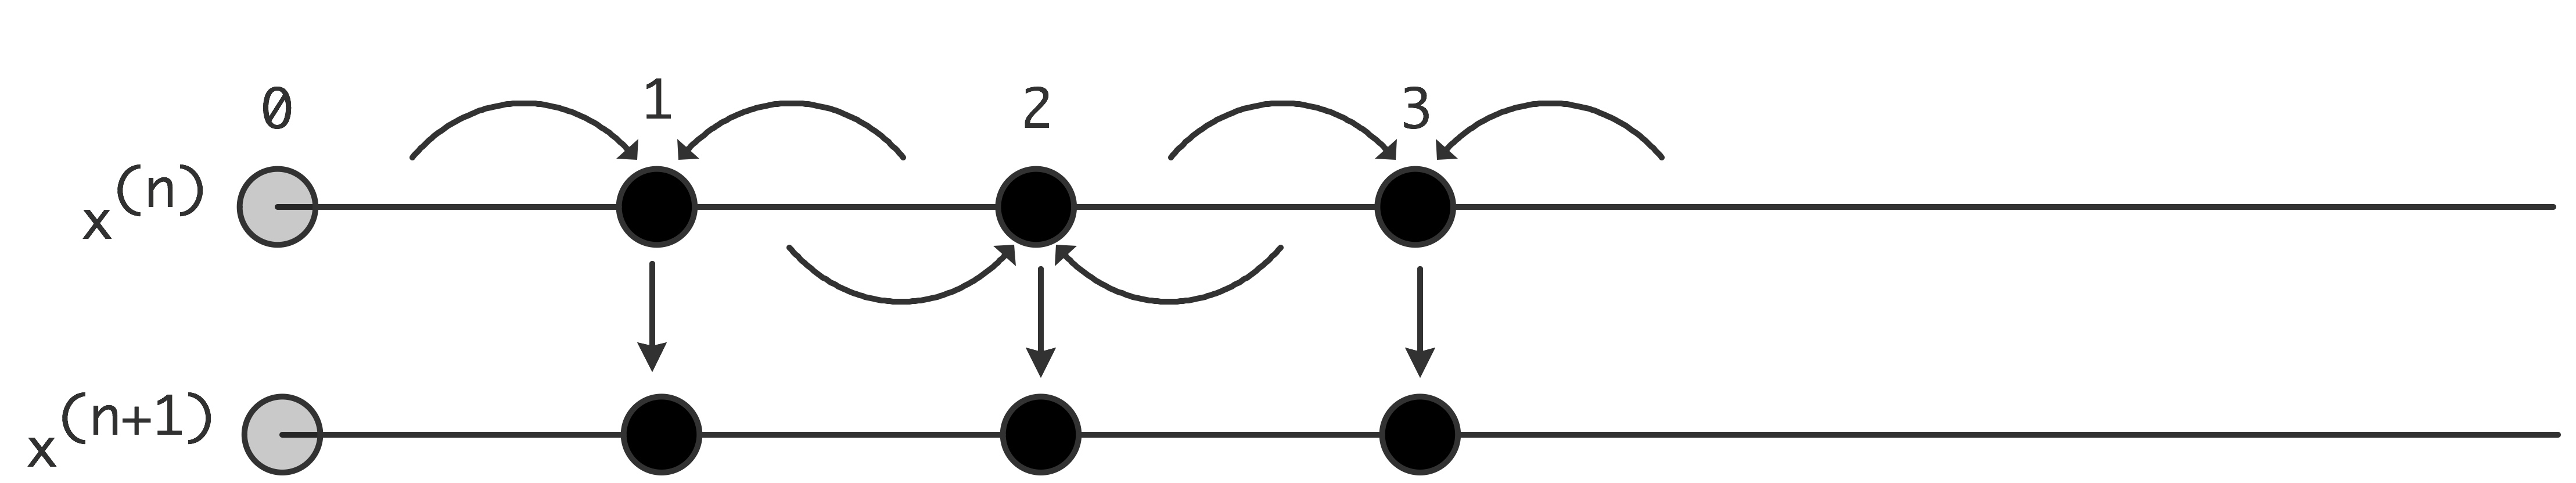
\includegraphics[scale=.08]{graphics/jacobi}
}

\frame{\frametitle{Gauss-Seidel}
\[ K=D_A+L_A \]
Algorithm:
\begin{quote}
  \begin{tabbing}
    for \=$k=1,\ldots$ until convergence, do:\\
    \>for \=$i=1\ldots n$:\\
    \>\>$//a_{ii}x^{(k+1)}_i +\sum_{j<i} a_{ij}x_j^{(k+1)}) =
                      \sum_{j>i} a_{ij}x_j^{(k)}+b_i\Rightarrow$\\
    \>\>$x^{(k+1)}_i = a_{ii}\inv (-\sum_{j<i} a_{ij}x_j^{(k+1)}) -
                      \sum_{j>i} a_{ij}x_j^{(k)}+b_i)$\\
  \end{tabbing}
\end{quote}
Implementation:
\begin{quote}
  \begin{tabbing}
    for \=$k=1,\ldots$ until convergence, do:\\
    \>for \=$i=1\ldots n$:\\
    \>\>$x_i = a_{ii}\inv (-\sum_{j\not=i} a_{ij}x_j +b_i)$\\
  \end{tabbing}
\end{quote}
}

\frame{\frametitle{GS in pictures:}
  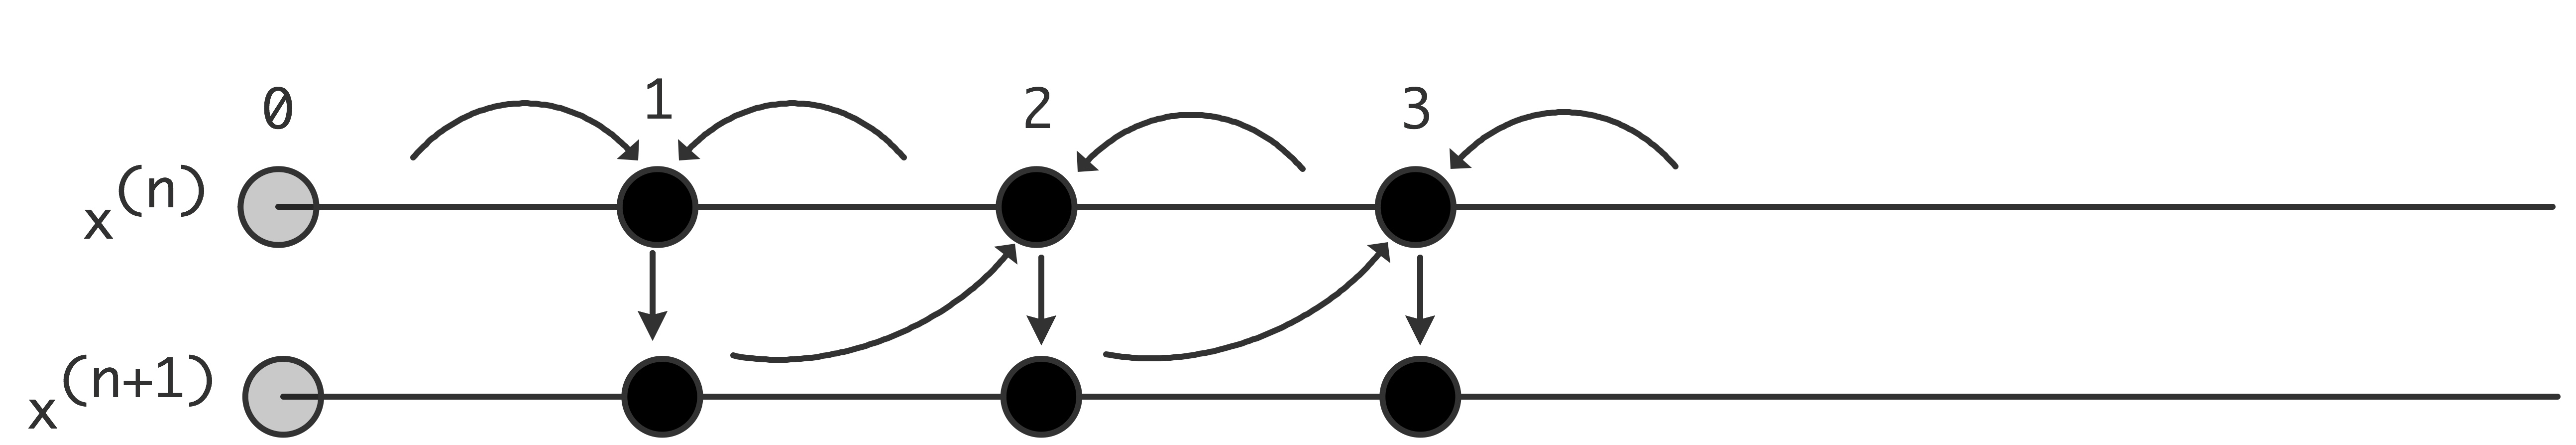
\includegraphics[scale=.08]{graphics/sor}
}

\frame[containsverbatim]{\frametitle{Choice of $K$ through incomplete LU}
  \begin{itemize}
  \item Inspiration from direct methods: let $K=LU\approx A$
  \end{itemize}
Gauss elimination:
\begin{verbatim}
for k,i,j:
   a[i,j] = a[i,j] - a[i,k] * a[k,j] / a[k,k]
\end{verbatim}
Incomplete variant:
\begin{verbatim}
for k,i,j:
  if a[i,j] not zero:
    a[i,j] = a[i,j] - a[i,k] * a[k,j] / a[k,k]
\end{verbatim}
$\Rightarrow$ sparsity of $L+U$ the same as of $A$
}

\frame[containsverbatim]{\frametitle{Stopping tests}
When to stop converging? Can size of the error be guaranteed?
  \begin{itemize}
  \item Direct tests on error $e_n=x-x_n$ impossible; two choices
  \item Relative change in the computed solution small:
    \[ \| x_{n+1}-x_n\|/\|x_n\|<\epsilon \]
  \item Residual small enough:
    \[ \|r_n\|=\|Ax_n-b\|<\epsilon \]
  \end{itemize}
  Without proof: both imply that the error is less than some
  other~$\epsilon'$.  }

\frame{\frametitle{General form of iterative methods 1.}

System $Ax=b$ has the same solution as $K\inv Ax=K\inv b$.

Let $\tilde x$ be a guess and
\[ \tilde r = K\inv A\tilde x-K\inv b. \]
then
\[ x=A\inv b=\tilde x-A\inv K\tilde r = \tilde x-(K\inv A)\inv \tilde r. \]
}

\frame{\frametitle{A little linear algebra}
Cayley-Hamilton theorem: 
\[ \hbox{$A$ nonsingular} \Rightarrow \exists_\phi\colon
 \phi(A)=\nobreak0 .\]
Write
\[ \phi(x)=1+x\pi(x), \]
Apply this to $K\inv A$:
\[
  0 = \phi( K\inv A ) = I + K\inv A \pi( K\inv A ) 
  \Rightarrow
  (K\inv A)\inv=-\pi(K\inv A)
\]
}
\frame{\frametitle{General form of iterative methods 2.}

Recall
\[ x= \tilde x-(K\inv A)\inv \tilde r. \]

Define iterates $x_i$ and residuals $r_i=Ax_i-b$, then
$\tilde r=K\inv r_0$.

Use Cayley-Hamilton:
\[ x=x_0-\pi(K\inv A)K\inv r_0= x_0-K\inv \pi(AK\inv) r_0. \]

so that $ x = \tilde x + \pi(K\inv A)\tilde r $. Now, if we let
$x_0=\tilde x$, then $\tilde r = K\inv r_0$, giving the equation
\[ x = x_0 + \pi(K\inv A)K\inv r_0 = x_0+K\inv \pi(AK\inv )r_0. \]
Iterative scheme:
\begin{equation}
  x_{i+1} = x_0+K\inv \pi^{(i)}(AK\inv) r_0
  \label{eq:x-from-PA-r0}
\end{equation}
}

\frame{\frametitle{Residuals}
\[   x_{i+1} = x_0+K\inv \pi^{(i)}(AK\inv) r_0 \]
Multiply by~$A$ and subtract~$b$:
\[ r_{i+1} = r_0+\tilde\pi^{(i)}(AK\inv)r_0 \]
So:
\[ r_i = \hat\pi^{(i)}(AK\inv) r_0 \]
where $\hat\pi^{(i)}$ is a polynomial of degree~$i$ with
$\hat\pi^{(i)}(0)=\nobreak1$. 

$\Rightarrow$ convergence theory
}

\frame{\frametitle{Juggling polynomials}

For $i=1$:
\[
  r_1 = (\alpha_1AK\inv+\alpha_2I)r_0 \Rightarrow 
  AK\inv r_0 = \beta_1r_1+\beta_0r_0
\]
for some values $\alpha_i,\beta_i$. 

For $i=2$
\[ r_2 = (\alpha_2(AK\inv )^2+\alpha_1AK\inv +\alpha_0)r_0 \]
for different values~$\alpha_i$. 

Together:
\[ (AK\inv)^2r_0\in \setspan{r_2,r_1,r_0}, \]
and inductively
\begin{equation}
  (AK\inv)^ir_0\in\setspan{r_i,\ldots,r_0}.
\end{equation}
}

\frame{\frametitle{General form of iterative methods 3.}
\[
  x_{i+1} = x_0 +\sum_{j\leq i} K\inv r_j\alpha_{ji}.
\]
or equivalently:
\[
  x_{i+1} = x_i +\sum_{j\leq i} K\inv r_j\alpha_{ji}.
\]
}

\frame{\frametitle{More residual identities}

\[
  x_{i+1} = x_i +\sum_{j\leq i} K\inv r_j\alpha_{ji}.
\]
gives
\[
  r_{i+1} = r_i+\sum_{j\leq i}AK\inv r_j\alpha_{ji}.
\]
Specifically
\[ r_1=r_0+AK\inv r_0\alpha_{00}. \]
so $AK\inv r_0 = \alpha_{00}\inv(r_1-r_0)$.

Next:
\[
\begin{array}{rl}
  r_2&=r_1+AK\inv r_1\alpha_{11}+AK\inv r_0\alpha_{01}\\
  &=r_1+AK\inv r_1\alpha_{11}+\alpha_{00}\inv\alpha_{01}(r_1-r_0)\\
  \Rightarrow AK\inv r_1&=\alpha_{11}\inv
  (r_2-(1+\alpha_{00}\inv\alpha_{01})r_1+\alpha_{00}\inv\alpha_{01}r_0)
\end{array}
\]
so $AK\inv r_1 = r_2\beta_2+r_1\beta_1+r_0\beta_0$, and that
$\sum_i\beta_i=0$. 
}

\frame{
Inductively:
\small
\[ 
\begin{array}{rll}
  r_{i+1}&=r_i+AK\inv r_i\delta_i+\sum_{j\leq i+1}r_j\alpha_{ji}\\
  r_{i+1}(1-\alpha_{i+1,i})&=AK\inv r_i\delta_i +r_i(1+\alpha_{ii})
      +\sum_{j< i} r_j\alpha_{ji}\\
  r_{i+1}\alpha_{i+1,i}&=AK\inv r_i\delta_i +
      \sum_{j\leq i}r_j\alpha_{ji}
      &\kern-40pt
       \vtop{
        \hbox{substituting $\begin{array}{ll}\alpha_{ii}:=1+\alpha_{ii}\\
        \alpha_{i+1,i}:=1-\alpha_{i+1,i}\end{array}$}
        \hbox{note that $\alpha_{i+1,i}=\sum_{j\leq i}\alpha_{ji}$}
        }\\
  r_{i+1}\alpha_{i+1,i}\delta_i\inv&=AK\inv r_i +\sum_{j\leq i}
  r_j\alpha_{ji}\delta_i\inv\\  
  r_{i+1}\alpha_{i+1,i}\delta_i\inv&=AK\inv r_i +\sum_{j\leq i}
      r_j\alpha_{ji}\delta_i\inv\\
  r_{i+1}\gamma_{i+1,i}&AK\inv r_i+\sum_{j\leq i} r_j\gamma_{ji}
      &\kern-40pt
       \hbox{substituting $\gamma_{ij}=\alpha_{ij}\delta_j\inv$}
\end{array}
\]
and we have that $\gamma_{i+1,i}=\sum_{j\leq i}\gamma_{ji}$.
}

\frame{\frametitle{General form of iterative methods 4.}
\[
  r_{i+1}\gamma_{i+1,i}=AK\inv r_i+\sum_{j\leq i} r_j\gamma_{ji}
\]
and $\gamma_{i+1,i}=\sum_{j\leq i}\gamma_{ji}$.

Write this as $AK\inv R=RH$ where
\[ H=
\begin{pmatrix}
  -\gamma_{11}&-\gamma_{12}&\ldots\\
  \gamma_{21}&-\gamma_{22}&-\gamma_{23}&\ldots\\
  0&\gamma_{32}&-\gamma_{33}&-\gamma_{34}\\
  \emptyset&\ddots&\ddots&\ddots&\ddots
\end{pmatrix}
\]
$H$ is a Hessenberg matrix, and note zero column sums.

Divide $A$ out:
\[
  x_{i+1}\gamma_{i+1,i}=K\inv r_i+\sum_{j\leq i} x_j\gamma_{ji}
\]
}

\frame{\frametitle{General form of iterative methods 5.}
\[
  \begin{cases}
    r_i = Ax_i-b\\
    x_{i+1}\gamma_{i+1,i}=K\inv r_i+\sum_{j\leq i} x_j\gamma_{ji}\\
    r_{i+1}\gamma_{i+1,i}=AK\inv r_i+\sum_{j\leq i} r_j\gamma_{ji}
  \end{cases}\qquad
  \hbox{where $\gamma_{i+1,i}=\sum_{j\leq i}\gamma_{ji}$}.
\]
}

\frame{\frametitle{Orthogonality}
Idea one:
\begin{quote}
  If you can make all your residuals orthogonal to each other, and the
  matrix is of dimension~$n$, then after $n$ iterations you have to
  have converged: it is not possible to have an $n+1$-st residuals
  that is orthogonal and nonzero.
\end{quote}
Idea two:
\begin{quote}
  The sequence of residuals spans a series of subspaces of increasing
  dimension, and by orthogonalizing the initial residual is projected on
  these spaces. This means that the errors will have decreasing sizes.
\end{quote}
}

\frame{
  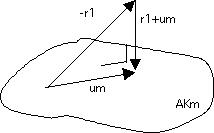
\includegraphics[scale=.7]{graphics/projection}
}

\frame{\frametitle{Full Orthogonalization Method}

\begin{quote}
  \begin{tabbing}
    Let $r_0$ be given\\
    For \=$i\geq 0$:\\
    \>let $s\leftarrow K\inv r_i$\\
    \>let $t\leftarrow AK\inv r_i$\\
    \>for \=$j\leq i$:\\
    \>\>let $\gamma_j$ be the coefficient so that $t-\gamma_jr_j\perp r_j$\\
    \>for \=$j\leq i$:\\
    \>\>form \=$s\leftarrow s-\gamma_jx_j$\\
    \>\>and  \>$t\leftarrow t-\gamma_jr_j$\\
    \>let $x_{i+1}=(\sum_j\gamma_j)\inv s$,
    $r_{i+1}=(\sum_j\gamma_j)\inv t$.\\
  \end{tabbing}
\end{quote}
}
\frame{\frametitle{Modified Gramm-Schmidt}
\begin{quote}
  \begin{tabbing}
    Let $r_0$ be given\\
    For \=$i\geq 0$:\\
    \>let $s\leftarrow K\inv r_i$\\
    \>let $t\leftarrow AK\inv r_i$\\
    \>for \=$j\leq i$:\\
    \>\>let $\gamma_j$ be the coefficient so that $t-\gamma_jr_j\perp r_j$\\
    \>\>form \=$s\leftarrow s-\gamma_jx_j$\\
    \>\>and  \>$t\leftarrow t-\gamma_jr_j$\\
    \>let $x_{i+1}=(\sum_j\gamma_j)\inv s$,
    $r_{i+1}=(\sum_j\gamma_j)\inv t$.\\
  \end{tabbing}
\end{quote}
}

\frame{\frametitle{Practical differences}
  \begin{itemize}
  \item Modfied GS more stable
  \item Inner products are global operations: costly
  \end{itemize}
}

\frame{\frametitle{Coupled recurrences form}

\begin{equation}
   x_{i+1}=x_i-\sum_{j\leq i}\alpha_{ji}K\inv r_j
   \label{eq:it-general-x}
\end{equation}
This equation is often split as
\begin{itemize}
\item Update iterate with search direction:
  direction:
\[ x_{i+1}=x_i-\delta_i p_i, \]
\item Construct search direction from residuals:
  \[ p_i = K\inv r_i+\sum_{j<i}\beta_{ij} K\inv r_j. \]
  Inductively:
  \[ p_i = K\inv r_i+\sum_{j<i}\gamma_{ij} p_j, \]
\end{itemize}
}


\frame{\frametitle{Conjugate Gradients}
Basic idea:
\[ r_i^tK\inv r_j=0\quad\hbox{if $i\not=j$}. \]
Split recurrences:
\[
  \begin{cases}
    x_{i+1}=x_i-\delta_i p_i \\
    r_{i+1}=r_i-\delta_iA p_i \\
    p_i = K\inv r_i+\sum_{j<i}\gamma_{ij} p_j,
  \end{cases}
\]
}

\frame{\frametitle{Symmetric Positive Definite case}
  Three term recurrence is enough:
\[
  \begin{cases}
    x_{i+1}=x_i-\delta_i p_i \\
    r_{i+1}=r_i-\delta_iA p_i \\
    p_{i+1} = K\inv r_{i+1}+\gamma_i p_i
  \end{cases}
\]
}

\frame{\frametitle{Preconditioned Conjugate Gradietns}
\small
\input pcg
}

\frame{\frametitle{Observations on iterative methods}
  \begin{itemize}
  \item Conjugate gradients: constant storage and inner products;
    works only for symmetric systems
    \item GMRES (like FOM): growing storage and inner products:
      restarting and numerical cleverness
    \item BiCGstab and QMR: relax the orthogonality
  \end{itemize}
}

\frame{\frametitle{CG derived from minimization}
Special case of SPD:
\begin{equation}
  \hbox{For which vector $x$ with $\|x\|=1$ is $f(x)=1/2 x^tAx-b^tx$ minimal?}
\end{equation}
Taking derivative:
\[ f'(x) = Ax-b. \]
Update
\[ x_{i+1} = x_i+p_i\delta_i \]
optimal value:
\[ \delta_i = \argmin_\delta \| f(x_i+p_i\delta) \| 
=\frac{r_i^tp_i}{p_1^tAp_i} 
\]
Other constants follow from orthogonality.
}

\end{document}


